\section{Problem, Data, and Empirical Difficulty}
\label{sec:data}
For a finite MDP $M=(S,A,P,R,\gamma,\rho)$, a logging behavior policy $\beta$, and a specified offline learner $l$, we ask whether a pilot log $D_0$ predicts the amount of \emph{additional, independently collected training data} that $l$ needs to reach a target return. Difficulty is the resulting learner- and behavior-conditional empirical data requirement. It is not a scalar property of $M$ alone or a theoretical sample-complexity bound.

Our registered experiment uses $\gamma=.95$, a pilot of $10|S||A|$ transitions, and training budgets $N_j=j|S||A|$ for $j\in\{1,2,5,10,20,50\}$. The policy-quality target uses normalized return
\begin{equation}
 {\rm NR}(\pi)=\frac{J(\pi)-J_{\rm random}}{J^*-J_{\rm random}}.
 \label{eq:nr}
\end{equation}
The output $E_l$ is the first measured budget where at least eight of ten independently trained seeds achieve ${\rm NR}\geq .95$ at that budget and every larger measured budget. Its seven categories are the six budgets and $>x50$; the last is right censoring, not an observed infinite requirement. Exact random and optimal returns define the \emph{evaluation label} in simulation; neither is supplied as a pilot-only forecast feature. The pilot itself costs $x10$, so predicted $x1$--$x5$ categories describe an independent training stream retrospectively, not prospective savings before pilot collection.

The same pilot can imply different empirical requirements for different learners. Missing important actions or rarely visited states reduce coverage, while stochastic transitions increase uncertainty in value estimates; BC, CFQI, and IQL respond differently to these conditions. Consequently, the target is $E_l(M,\beta,.95)$ for a specified learner, behavior, and threshold, rather than one intrinsic difficulty score for the dataset. The six measured budgets form a grid: $E_l$ does not identify the exact number of transitions needed between grid points.

Figure~\ref{fig:pipeline} separates the pilot-only forecast path from the independent training streams that supply evaluation labels. This separation is essential: the oracle references used to score policy return and the measured budget outcomes are unavailable to the forecaster at test time.

\begin{figure*}[t]
\centering
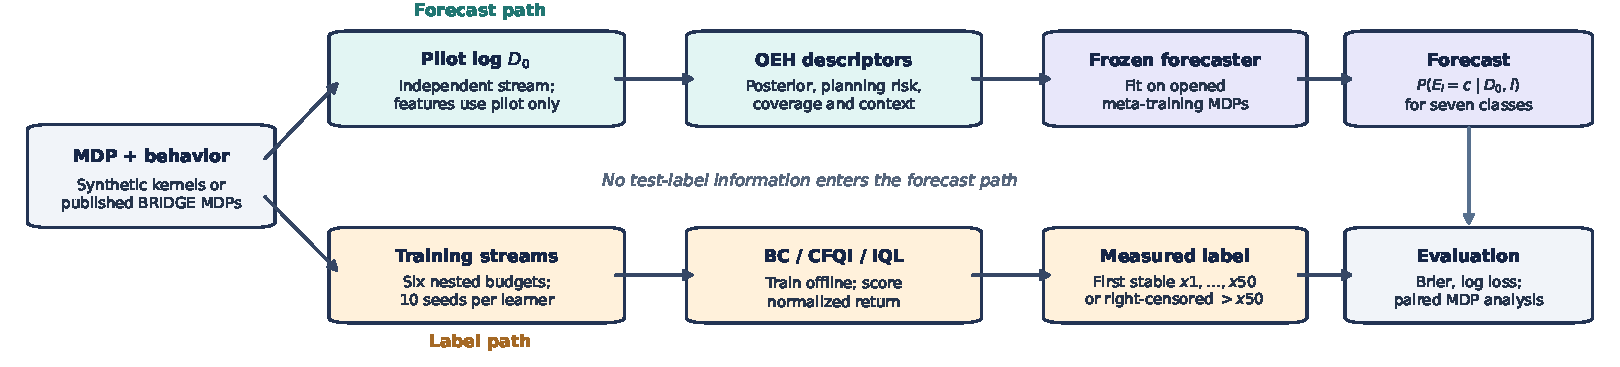
\includegraphics[width=\textwidth]{figures/oeh_pipeline.pdf}
\caption{Study pipeline. Each test MDP and behavior policy yields an independent pilot and training streams. OEH features and the frozen forecaster see the pilot and learner identity, while six budget levels and ten training seeds establish the measured, possibly right-censored requirement label. Brier and log loss compare forecasts and labels on identical test rows; uncertainty is clustered by MDP. The published BRIDGE MDPs supply environments, not author-provided offline requirement labels.}
\label{fig:pipeline}
\end{figure*}

\textbf{Why the controlled data are generated.} Observing this target requires multiple budgets and seeds for the same MDP--behavior--learner combination, an independent pilot, and reliable random and optimal return references. The sealed panel contains 120 new MDP kernels: 84 stochastic Garnet, forward-layered, and bottleneck instances for primary analysis and 36 deterministic lock controls. State/action counts, branching, transition concentration, reward sparsity, and bottleneck structure follow preregistered stratified recipe levels, with new hash-derived kernel seeds. The common ex-ante return-span filter rejected three bottleneck proposals; it never inspected OEH predictions or learner outcomes. Each MDP has five registered behavior policies; one uses oracle information \emph{only to generate the logged behavior}, which is disclosed and excluded from pilot-only features. For each MDP--behavior pair, one pilot stream and ten independent training streams are generated under separate seed namespaces. Budgets are nested prefixes of each training stream, not independent datasets. Every method sees the same accepted kernels, pilot rows and label rule, but this matching does not eliminate bias from familiar generator families, oracle-informed behavior generation, or the return-span filter. Transfer to independently designed MDPs is evaluated separately.

Published stochastic environments and offline datasets do exist. Our controlled panel is generated because the registered $E_l$ label needs six matched budgets, ten training seeds, and exact return references for each learner and behavior policy. The independently published BRIDGE MDPs provide a separate environment test; the offline pilot logs and $E_l$ labels used there are collected by our protocol, not supplied as a published offline dataset by the BRIDGE authors.

\textbf{Why these learners.} The primary requirement grid uses behavior cloning (BC) as an imitation baseline, the project's conservative fitted Q-iteration (CFQI) as a value-based offline learner, and implicit Q-learning (IQL) as an offline value/policy alternative~\cite{kostrikov2022iql}. All train from fixed logs; the three-way choice provides distinct responses to coverage and policy quality while keeping the multi-budget, ten-seed label experiment feasible. Four additional learners appear only in the secondary single-budget selection experiment (Section~\ref{sec:selection}); their returns are not extra requirement targets.
